\documentclass{beamer}
 
\usepackage[utf8]{inputenc}
\usepackage[english]{babel}
\usepackage{amsmath}
\usepackage{amsfonts}
\usepackage{amssymb}
\usepackage{graphicx} 
\usepackage{latexsym} 
\usepackage{listings}
\usepackage{xcolor}
\usepackage{soul}
\usepackage[T1]{fontenc}
\usepackage{amsthm}
\usepackage{mathtools}
\usepackage{setspace}
\usepackage{array,multirow,makecell}
\usepackage{geometry}
\usepackage{textcomp}
\usepackage{float}
\usepackage{bbold}
\usepackage{wrapfig}
\usepackage{textpos}

\rmfamily

\usetheme{Madrid}
%%\usecolortheme{beaver}



\title{LC 24 Diagrammes potentiel PH}
\institute{Université Paul sabatier}
\date{Agrégation 2019}

 
\begin{document}
	
\begin{frame}
	\titlepage
\end{frame}

\addtocounter{framenumber}{-1}
\title{Diagrammes potentiel PH}

\begin{frame}
\frametitle{Diagramme potentiel PH de l'eau}
\begin{figure}[H]
	\centering
		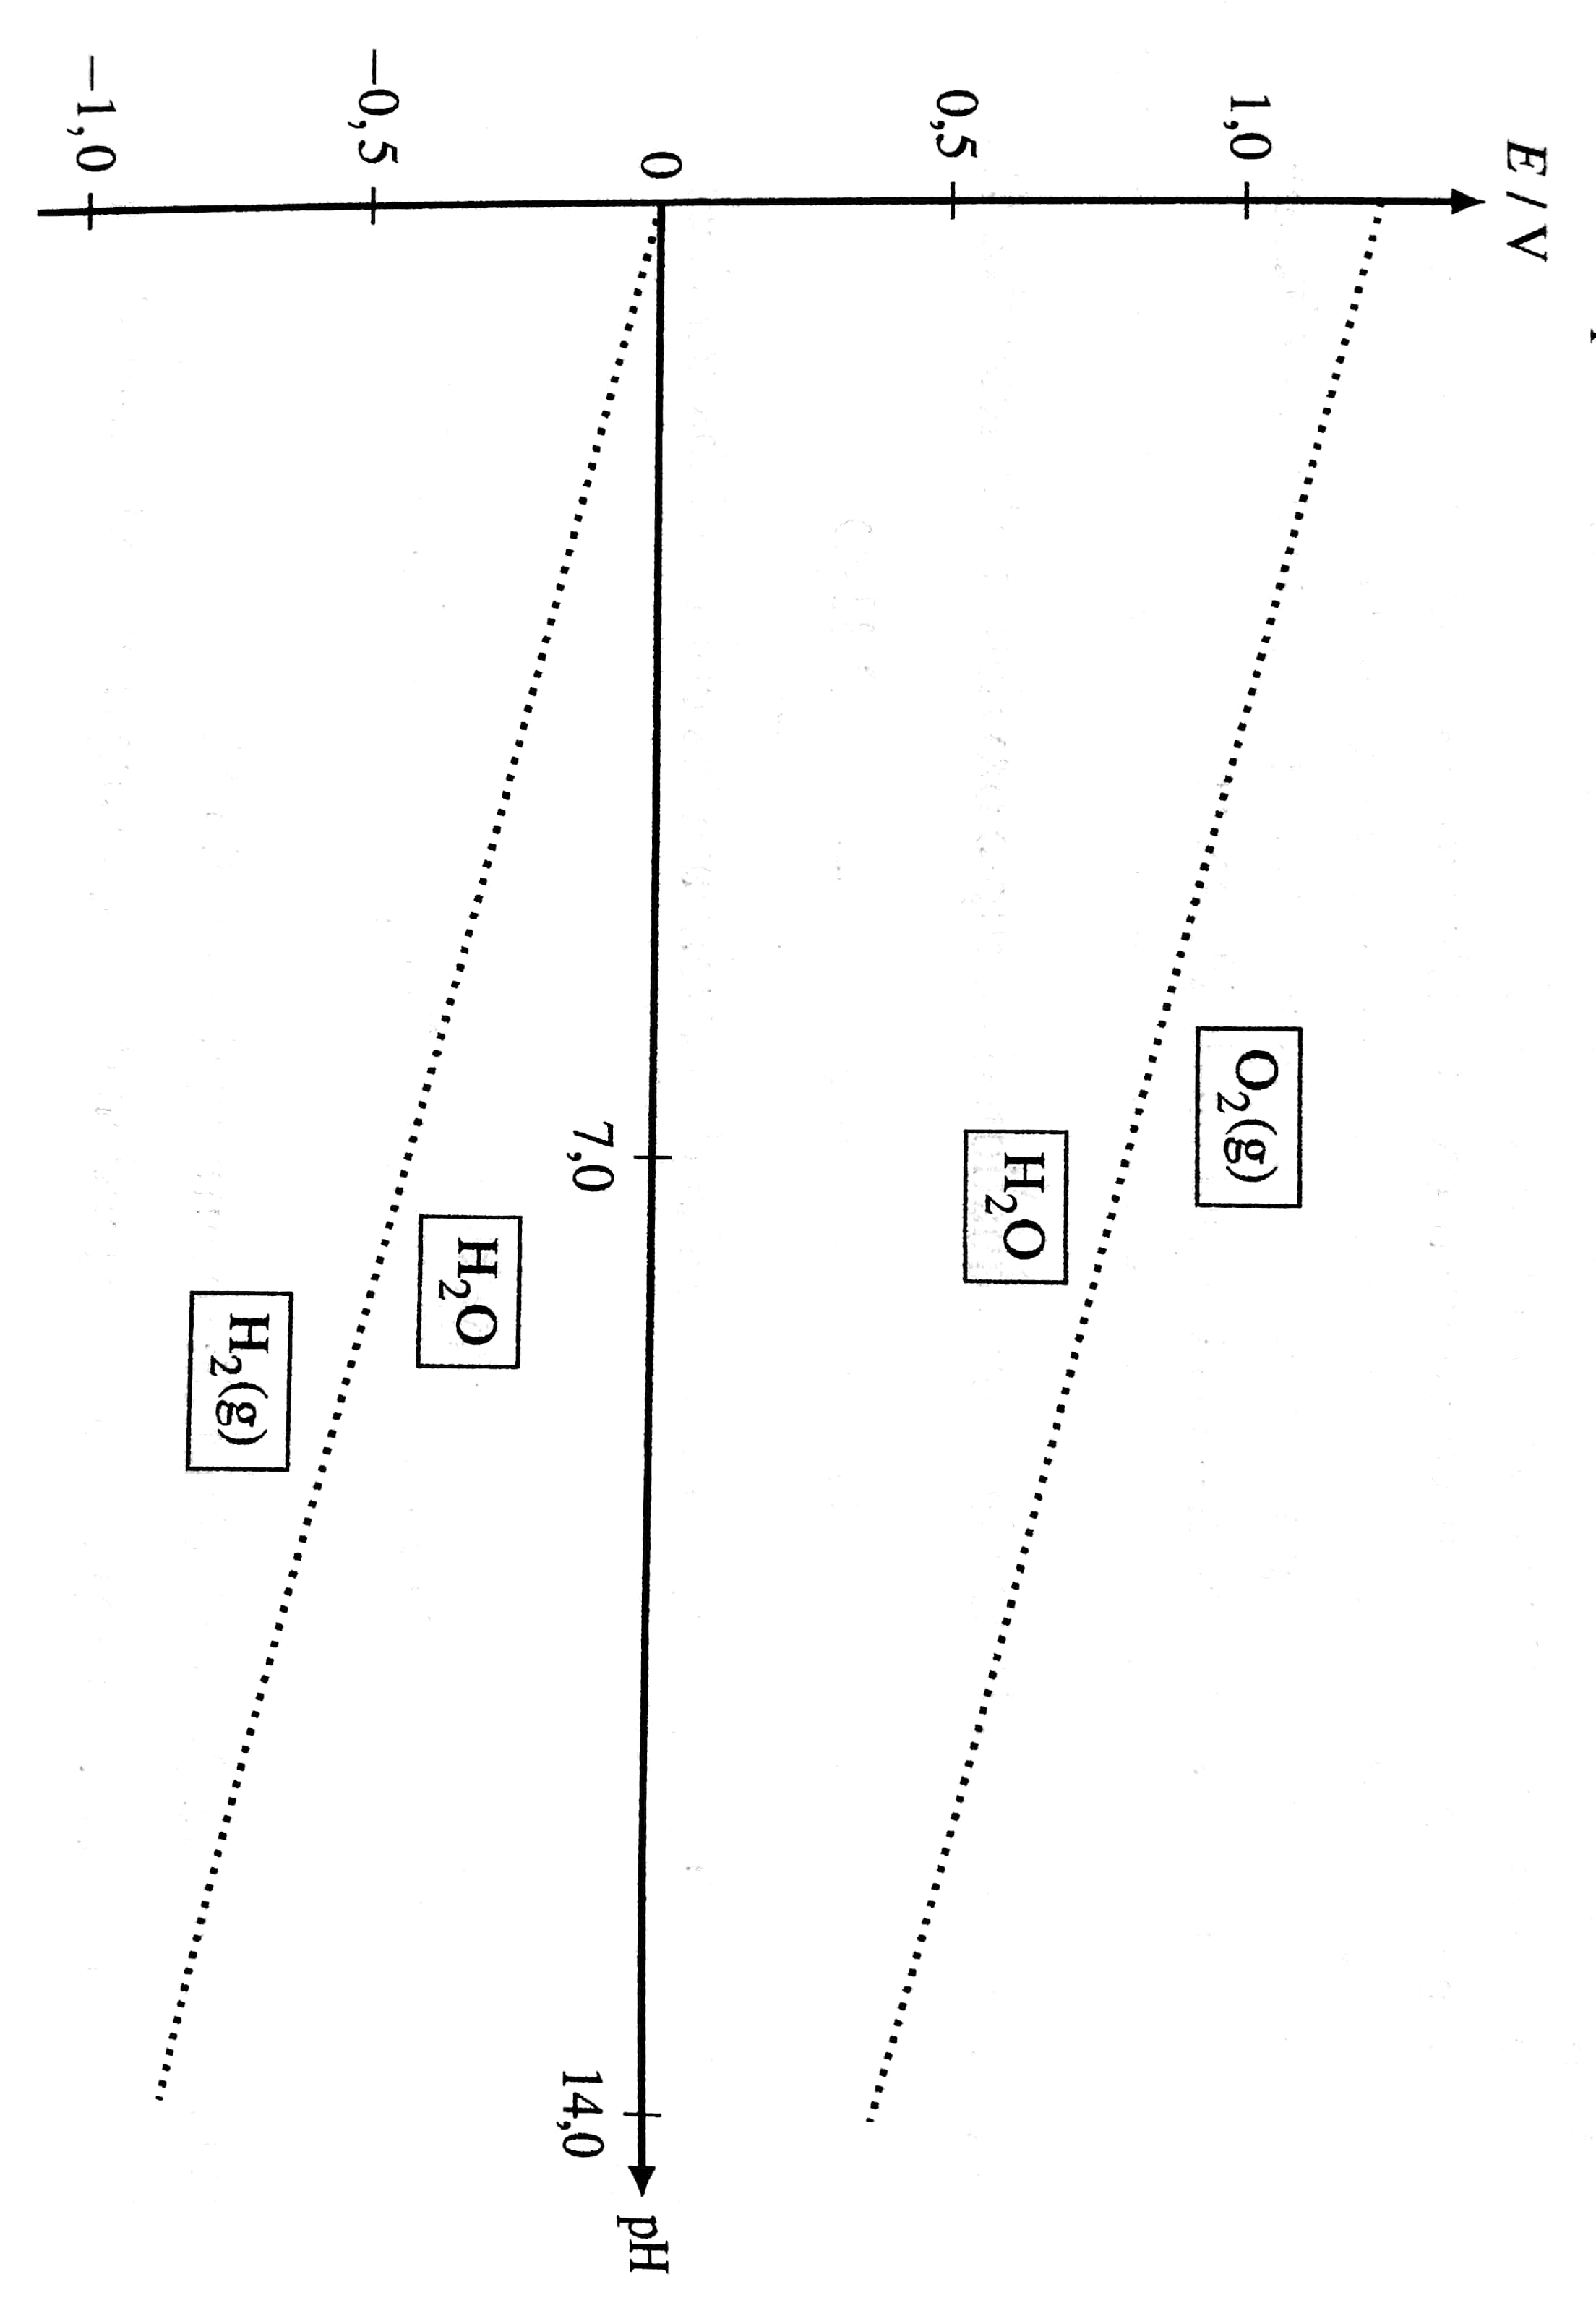
\includegraphics[width=6cm, angle=90]{eau}
\end{figure}
Pression de tracé $P=1$ bar, construit pour T=298K.
\end{frame}

\begin{frame}
\frametitle{Diagramme potentiel PH du fer}
\begin{figure}
	\centering 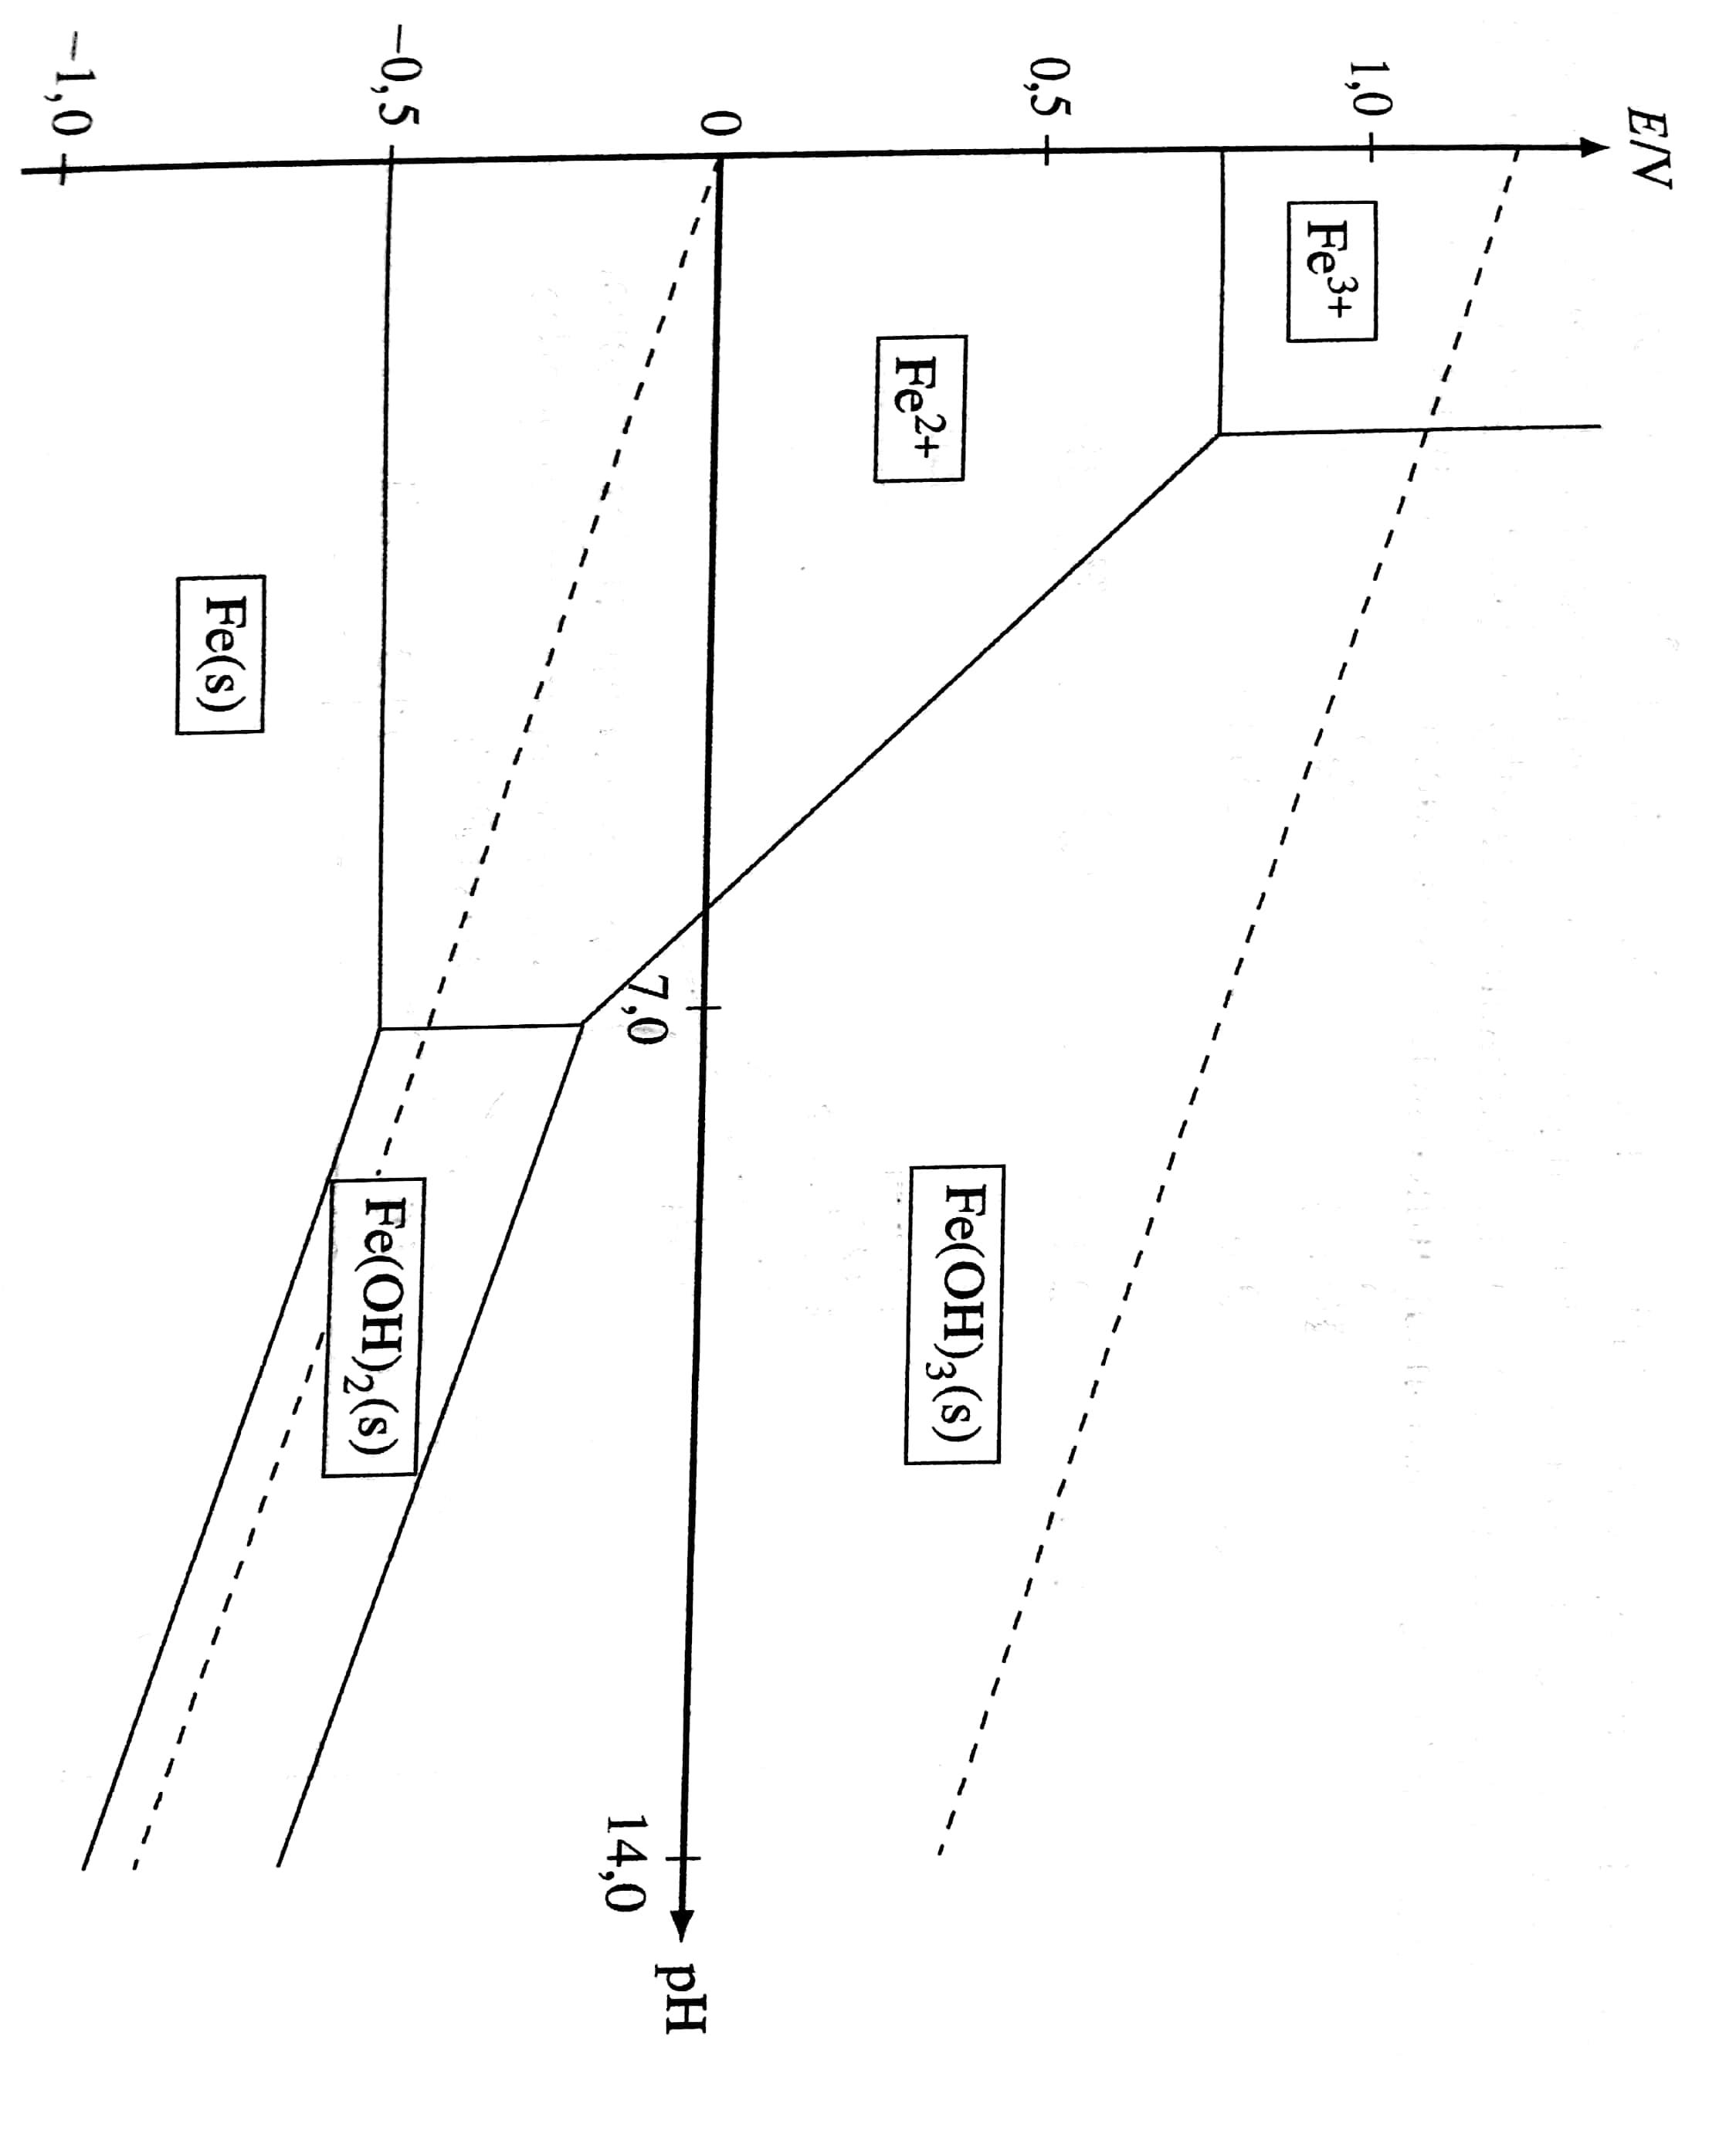
\includegraphics[width=6cm, angle=90]{fer}
\end{figure}
Concentration de tracé $C=10^{-2}$ mol.L$^{-1}$, construit pour T=298K.
\end{frame}

\begin{frame}
\frametitle{Diagramme potentiel PH du zinc}
\begin{figure}[H]
	\centering
	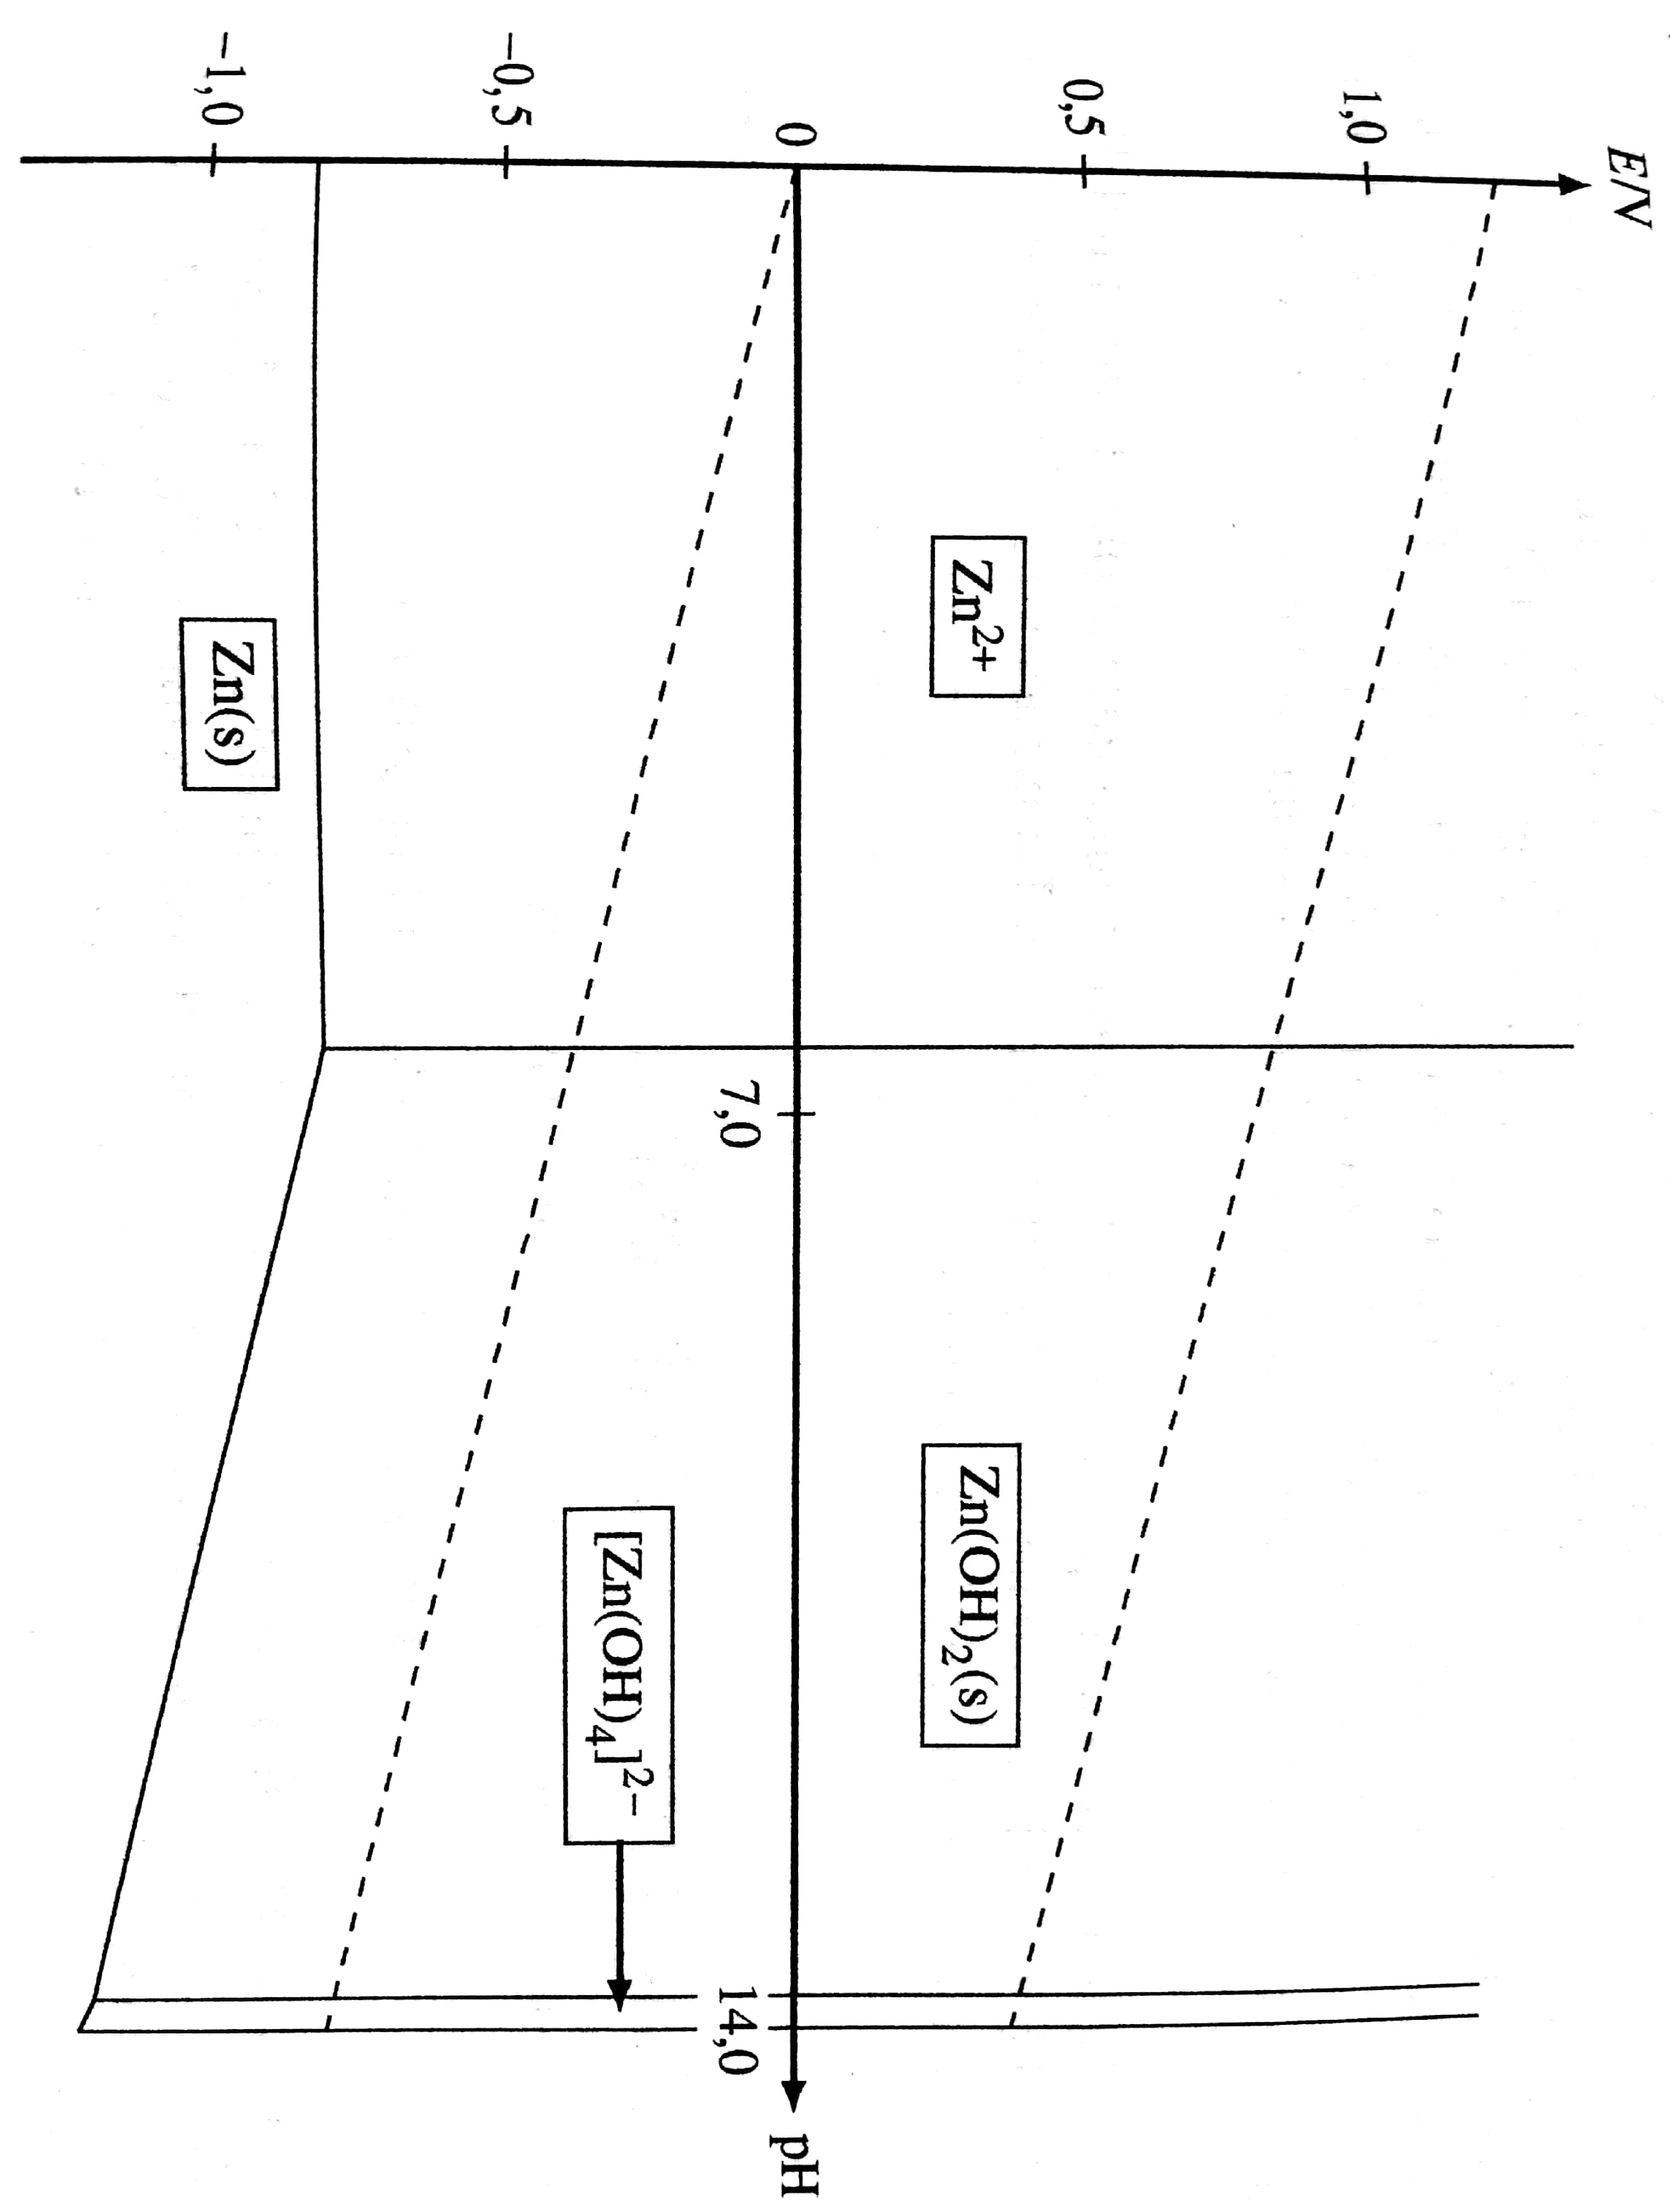
\includegraphics[width =6cm, angle=90]{zinc}
\end{figure}
Concentration de tracé $C=10^{-2}$ mol.L$^{-1}$, construit pour T=298K.
\end{frame}

\end{document}